\documentclass[letterpaper, 11pt]{amsart}

\usepackage{fullpage}
\usepackage{graphicx}
\usepackage{amsmath, amssymb, amsfonts}

\usepackage{color}
\usepackage[colorlinks=true,linkcolor=red,citecolor=blue,urlcolor=cyan]{hyperref}

\definecolor{crimsonred}{RGB}{190,0,0}
\definecolor{granitepeak}{RGB}{117,142,153}
\definecolor{lakecolor}{RGB}{58,191,192}

\newcommand{\red}[1]{\textcolor{crimsonred}{#1}}
\newcommand{\DAR}[1]{\textcolor{granitepeak}{#1}}
\newcommand{\replace}[1]{\textcolor{lakecolor}{#1}}
\newcommand{\BO}[1]{\textcolor{blue}{\small {\sf BO:\@ #1}}}


\begin{document}
\noindent {\bf Robert Stutchbury \\ 
Math 5750/6880: Mathematics of Data Science \\  
Project \#2 Final Report \\ 
\today \\ }


\noindent My GitHub Project2 repository is located here:
\begin{center}
    \url{https://github.com/kerbs23/F25_math_for_data_science/tree/main/projects/Project2}
\end{center}


%%%%%%%%%%%%%%%%%%%%%%%%%%%%%%%%%%
\section{Clustering Gaussian Blobs using k-means}

This one was fairly easy and peasy. Did it with the 5 clusters first, then modified it a little so that I could put it into a loop for the elbow analysis.
The PCA down to 2 dimensions seems to separate things nicely, but leaves two of the blobs roughly stacked on top of each other.

\begin{figure}[h]
\centering
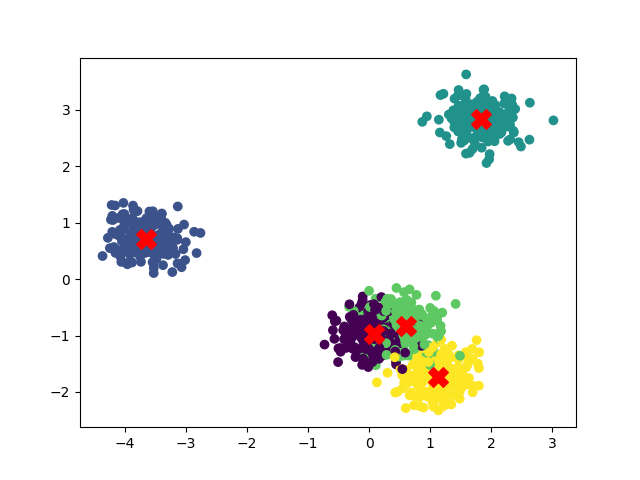
\includegraphics[width=0.8\textwidth]{plots/KMeans_plot.png}
\caption{K-means clustering results on 2D Gaussian blobs showing cluster assignments and centroids}
\end{figure}

This makes sense, if the blobs are nicely separated in a higher dimension, each var maximising dim in the pca should roughly spread the blobs out in half, if not randomly be able to do a bit better.
Actually, here: The Bob Conjecture: For a bunch of well separated high-dim blobs, pca down to $n$ dim s.t. $$2^n < number of blobs$$ will leave you able to cleanly identify all the clusters.
Too vague to prove but still interesting to think about.



To match the clusters for the confusion matrix, I just did a simple mode: for each kmeans label, whichever actual label appears the most is given its match.
Then, we just rewrite the entire column to its mode and we can use the built-in sklearn library to make the matrix.

\begin{tabular}{rrrrr}
\toprule
\midrule
200 & 0 & 0 & 0 & 0 \\
0 & 200 & 0 & 0 & 0 \\
0 & 0 & 200 & 0 & 0 \\
0 & 0 & 0 & 200 & 0 \\
0 & 0 & 0 & 0 & 200 \\
\bottomrule
\end{tabular}

Very nice.

Finally, the elbow analysis for k-means:
\begin{figure}[h]
\centering
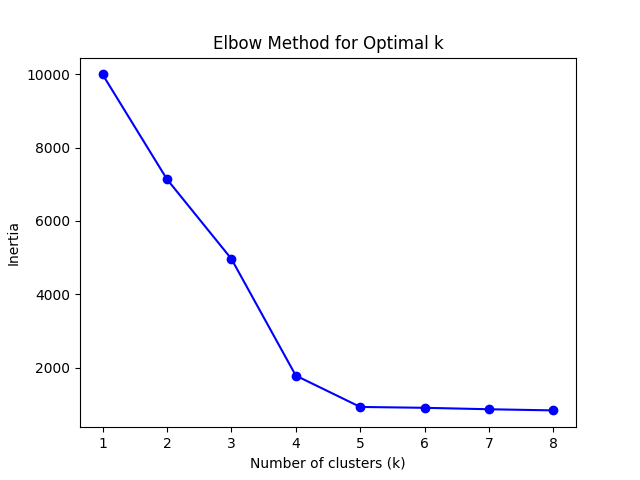
\includegraphics[width=0.8\textwidth]{plots/elbow_plot.png}
\caption{Elbow plot showing optimal k value selection for k-means clustering on Fashion-MNIST data}
\end{figure}


%%%%%%%%%%%%%%%%%%%%%%%%%%%%%%%%%%
\section{Clustering Fashion-MNIST using k-means}

Just did what I did above, with the technical difference of not using a pd df to help keep things straight.

\begin{figure}[h]
\centering
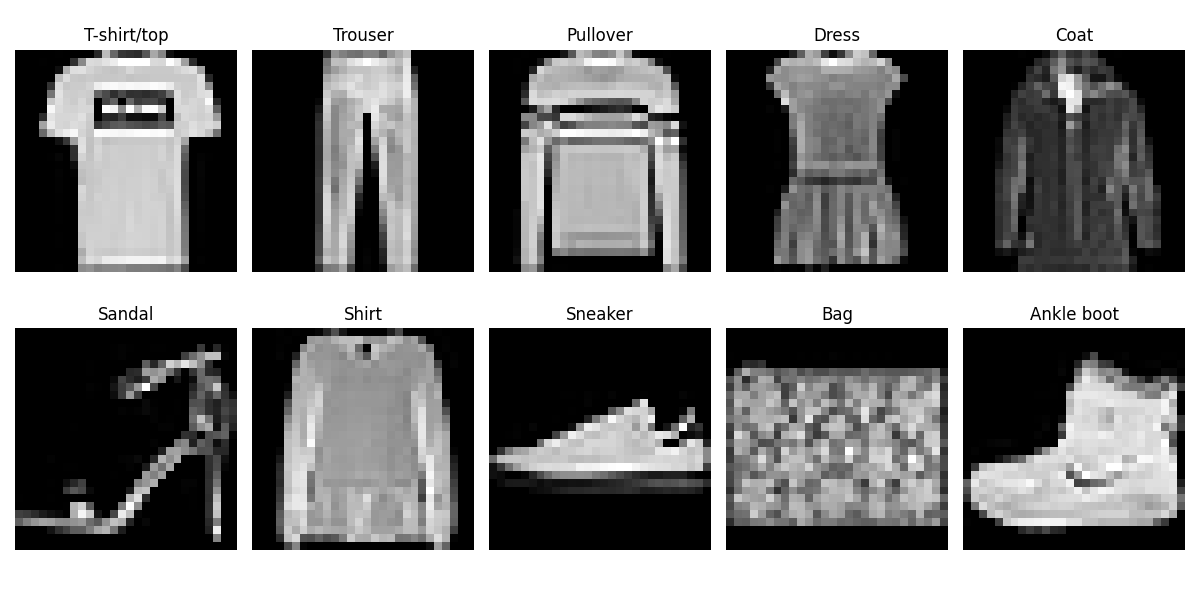
\includegraphics[width=0.8\textwidth]{plots/examble_items_fashion.png}
\caption{Example items from the Fashion-MNIST dataset showing various clothing categories}
\end{figure}

The k-means did not do as well as the previous much simpler example.

\begin{tabular}{lrrrrrrrrrr}
\toprule
 & T-shirt/top & Trouser & Pullover & Dress & Coat & Sandal & Shirt & Sneake
r & Bag & Ankle boot \\
\midrule
T-shirt/top & 3201 & 63 & 0 & 1166 & 64 & 435 & 1999 & 5 & 67 & 0 \\
Trouser & 17 & 6154 & 0 & 443 & 62 & 121 & 198 & 0 & 5 & 0 \\
Pullover & 218 & 7 & 0 & 196 & 3958 & 421 & 2091 & 5 & 103 & 1 \\
Dress & 52 & 2605 & 0 & 2968 & 49 & 415 & 905 & 0 & 5 & 1 \\
Coat & 11 & 73 & 0 & 1351 & 4125 & 220 & 1151 & 1 & 68 & 0 \\
Sandal & 0 & 0 & 0 & 4 & 0 & 4856 & 68 & 1529 & 9 & 534 \\
Shirt & 751 & 29 & 0 & 801 & 2096 & 707 & 2470 & 10 & 135 & 1 \\
Sneaker & 0 & 0 & 0 & 0 & 0 & 785 & 1 & 5959 & 0 & 255 \\
Bag & 70 & 10 & 0 & 95 & 116 & 394 & 627 & 473 & 5190 & 25 \\
Ankle boot & 2 & 1 & 0 & 24 & 12 & 241 & 64 & 974 & 4 & 5678 \\
\bottomrule
\end{tabular}

This pretty much tracks for me, since similar items like shoes and sandals get confused for each other more often than wildly different ones.

You can, however, see that my modal matching method did not match anything for the pullover, looks like this and the coat category got merged.
I see this as fine, since it just indicates coats and pullovers look similar, but pullovers are hard to identify so it's safer to just guess coats.
Reasonable people could disagree.

%%%%%%%%%%%%%%%%%%%%%%%%%%%%%%%%%%
\section{Dimensionality reduction for Fashion-MNIST}

Running this was not nice for my computer; specifically the pairwise distances.
\begin{figure}[h]
\centering
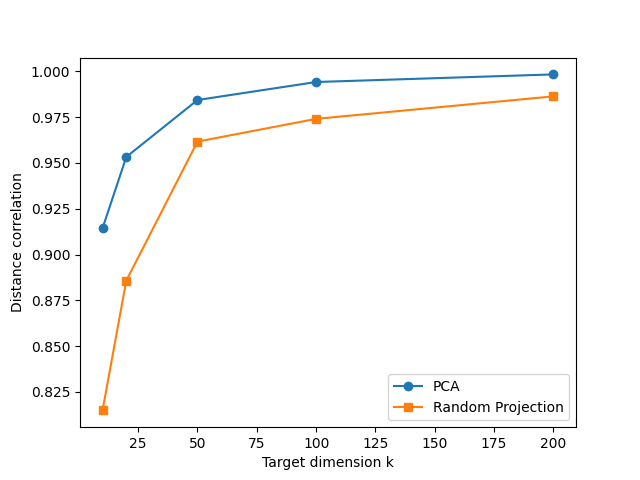
\includegraphics[width=0.8\textwidth]{plots/comparison_pca_vs_rand.png}
\caption{Comparison of PCA vs random projection dimensionality reduction performance on Fashion-MNIST}
\end{figure}
Ended up cutting down to a 10\% sample of the data, which is enough to sort of demonstrate the lemma.

Just loops over the sklearn built-in modules with different ks, taking the correlations and then graphing them. As usual, quite impressed with both the PCA and random dim reductions.

%%%%%%%%%%%%%%%%%%%%%%%%%%%%%%%%%%
\section{Clustering Fashion-MNIST using spectral clustering}

This was very hard on my computer. 
I PCAd the data down to 50 dims and took a 10\% sample, and even this was too much for my little thinkpad to handle,even leaving it churning for 5 hours while I cleaned my appartment.
I PCA'd the data down to 50 dims and took a 10\% sample, and even this was too much for my little ThinkPad to handle, even leaving it churning for 5 hours while I cleaned my apartment.
At the end, it just had one of the cores of my CPU at max always and like 75\% of my RAM pinned down, so I am not really sure what it was up to.
I spent a while trying to debug it, since it throws a weird error that the graph is disconnected even though with the graph creation method that should be impossible, and got no leads. 
This thing is already 2 days late though, so I am going to email it over, esp. since the analysis is just calling that confusion matrix function on the output and comparing its matrix with the k-means'.


\end{document}
